\documentclass[a4paper, 12pt]{article}

\newcommand{\templates}{../../../template}
\usepackage[a4paper, margin=2.5cm]{geometry}

\usepackage{enumitem}
\setlist[itemize]{noitemsep}
\setlist[enumerate]{noitemsep}

\let\oldpar\paragraph
\renewcommand{\paragraph}[1]{\oldpar{#1\\}\noindent}
\usepackage{graphicx}
\usepackage{hyperref}
\usepackage{makecell}

\newcommand{\settitolo}[1]{\newcommand{\titolo}{#1\\}}
\newcommand{\setprogetto}[1]{\newcommand{\progetto}{#1\\}}
\newcommand{\setcommittenti}[1]{\newcommand{\committenti}{#1\\}}
\newcommand{\setredattori}[1]{\newcommand{\redattori}{#1\\}}
\newcommand{\setrevisori}[1]{\newcommand{\revisori}{#1\\}}
\newcommand{\setresponsabili}[1]{\newcommand{\responsabili}{#1\\}}
\newcommand{\setversione}[1]{
	\ifdefined\versione\renewcommand{\versione}{#1\\}
	\else\newcommand{\versione}{#1\\}\fi
}
\newcommand{\setdestuso}[1]{\newcommand{\uso}{#1\\}}
\newcommand{\setdescrizione}[1]{\newcommand{\descrizione}{#1\\}}

\newcommand{\makefrontpage}{
	\begin{titlepage}
		\begin{center}

		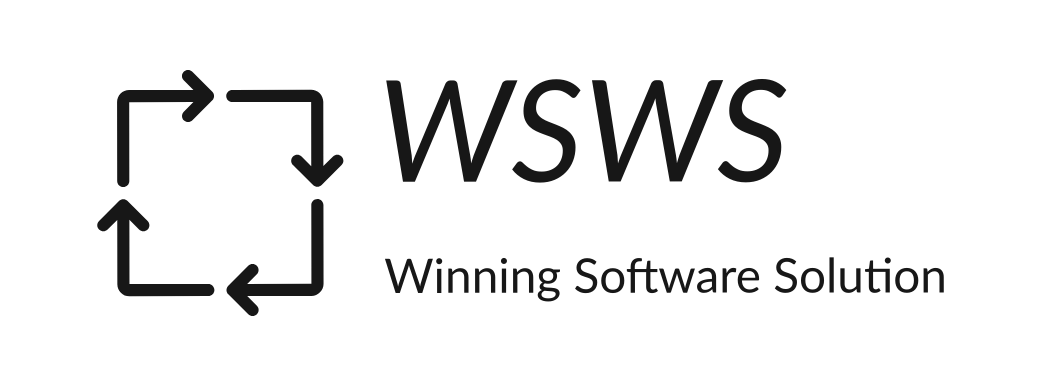
\includegraphics[width=0.4\textwidth]{../../template/WSWS-logos_transparent_crop}\\

		{\Large Winning Software Solution}\\[6pt]
		\href{mailto://winningsoftwaresolution@gmail.com}{winningsoftwaresolution@gmail.com}\\
		
		\ifdefined\progetto
		\vspace{1cm}
		{\Large\progetto}
		{\large\committenti}
		\else\fi
		
		\vspace{1.5cm}
		{\LARGE\titolo}
		
		\vfill
		
		\begin{tabular}{r | l}
		\multicolumn{2}{c}{\textit{Informazioni}}\\
		\hline
		
		\ifdefined\redattori
			\textit{Redattori} &
			\makecell[l]{\redattori}\\
		\else\fi
		\ifdefined\revisori
			\textit{Revisori} &
			\makecell[l]{\revisori}\\
		\else\fi
		\ifdefined\responsabili
			\textit{Respondabili} &
			\makecell[l]{\responsabili}\\
		\else\fi
		
		\ifdefined\versione
			\textit{Versione} & \versione
		\else\fi
		
		\textit{Uso} & \uso
		
		\end{tabular}
		
		\vspace{2cm}
		
		\ifdefined\descrizione
		Descrizione
		\vspace{6pt}
		\hrule
		\descrizione
		\else\fi
		\end{center}
	\end{titlepage}
}
\usepackage{hyperref}
\usepackage{array}
\usepackage{tabularx}

\def\vers#1-#2-#3-#4-#5\\{#1&#2&#3&#4&#5\\\hline}

\newcommand{\addversione}[5]{
	\ifdefined\versioni
		\let\old\versioni
		\renewcommand{\versioni}{#1&#2&#3&#4&#5\\\hline\old}
	\else
		\newcommand{\versioni}{#1&#2&#3&#4&#5\\\hline}
	\fi
}

\newcommand{\setversioni}[1]{\newcommand{\versioni}{#1}}

\newcommand{\makeversioni}{
	\begin{center}
		\begin{tabularx}{\textwidth}{|c|c|c|c|X|}
		\hline
		\textbf{Versione} & \textbf{Data} & \textbf{Persona} & \textbf{Attivtà} & \textbf{Descrizione} \\
		\hline
		\versioni
		\end{tabularx}
	\end{center}
	\clearpage
}

\settitolo{Verbale del 12/11/2021 con SyncLab}
\setredattori{Federico Marchi\\Elia Scandaletti}
\setrevisori{Andrea Volpe}
\setdestuso{interno}
\setdescrizione{
Verbale dell'incontro del 12/11/2021 con l'azienda SyncLab. 
}

\begin{document}

\makefrontpage

\section{Informazioni}
\textbf{Data}: 12/11/2021\\
\textbf{Durata}: 45 minuti\\
\textbf{Luogo}: Aula Virtuale Google Meet\\

\textbf{Partecipanti}
\begin{itemize}
	\item Andrea Volpe
	\item Giovanni Cocco
	\item Federico Marchi
	\item Alberto Nicoletti
	\item Matteo Galvagni
	\item Elia Scandaletti
	\item Fabio Pallaro
\end{itemize}

\section{Ordine del giorno}
\begin{enumerate}
	\item Domande da parte del gruppo al proponente;
	\item Varie ed eventuali.
\end{enumerate}

\section{Svolgimento}

\subsection{Domande da parte del gruppo al proponente}
Sono state richieste delucidazioni riguardo ad alcuni argomenti non chiari circa le richieste del proponente.

\begin{itemize}

\item \textbf{Cosa si intende per caricare il codice QR in blockchain?}
Abbiamo discusso sul fatto che il caricamento del QR code in blockchain sotto forma di stringa sia dispendioso (aumenta le fees della transazione) e non 	necessario. Dunque si è optato di risolvere il problema della verifica dell’identità dell’utente che scannerizza il codice QR richiedendo una sorta di login attraverso l’uso del medesimo wallet che ha effettuato il pagamento (quindi verificando che l’utente che scannerizza e che dunque sbloccherà i fondi nello smart contract sia realmente l’acquirente).

\item \textbf{Quali dati vanno caricati sul DB aziendale e quali invece in blockchain?}
In blockchain saranno presenti solamente i dati riguardanti la transazione e i wallet che l’hanno effettuata/ricevuta con data e ora. Non è importante essere a conoscenza dell’oggetto acquistato.
 Dunque la blockchain non avrà funzione di database, le altre informazioni relative all’acquisto saranno salvate su DB aziendale.

\item \textbf{Come viene gestita la visualizzazione dei vari ordini sulla pagina web? Sarà possibile visualizzare tutti gli ordini o solo il proprio?}
La pagina web deve permettere al venditore di visualizzare lo stato di ciascuna transazione (non necessariamente visualizzare a che punto e dove si trova il pacco durante la consegna). Sarà possibile, attraverso l’identificazione tramite il proprio wallet, visualizzare esclusivamente le transazioni che comprendono l’address di quel determinato wallet.

\item \textbf{Bisogna dare la possibilità di pagare con qualsiasi cryptovaluta o scegliere la valuta nativa della blockchain utilizzata?}
Si è riflettuto su questo punto arrivando alla conclusione che per semplicità conviene permettere il pagamento solo attraverso l’utilizzo della valuta nativa della blockchain utilizzata. Tuttavia un possibile plus è quello di permettere il pagamento con qualsiasi valuta compatibile con quella determinata blockchain per poi convertirla successivamente con l’ausilio di un exchange (attenzione però alle fees aggiuntive). 
Un altro punto su cui si è discusso è il frequente cambio di valore nel tempo (volatilità) di diverse valute. Questo potrebbe diventare un problema qualora nello smart contract venga bloccata una valuta molto volatile. Si è pensato ad una possibile soluzione ovvero quella di convertire tutti i pagamenti in valuta stabile prima di bloccare i fondi nello smart contract.
 
\item \textbf{Come è possibile garantire la sicurezza ed evitare che un “man in the middle” tra l’e-commerce e la landing page possa accedere alle informazioni del venditore?}
Durante la discussione è sorta una possibile soluzione: prima di ogni acquisto il server dell'e-commerce comunica al server BlockChange l'intenzione di ricevere un pagamento attraverso un canale criptato con sistema a chiave asimmetrica; in questo modo, qual'ora il server BlockChange ricevesse dall'utente finale una richiesta discordante, sarebbe in grado di individuare un attacco MitM. La necessità dell'e-commerce di possedere una chiave privata fornita da BlockChange permetterebbe anche di fornire il servizio selettivamente. Il contro della soluzione è l'e-commerce sarebbe costretto a modificare il proprio backend per renderlo compatibile.

\item \textbf{Come comportarsi in caso di eventuali contestazioni e come gestire lo sblocco del denaro nello smart contract?}
Si è pensato di reindirizzare all’e-commerce possibili contestazioni da parte dell’acquirente, tenendo conto della legge Europea riguardo la possibile restituzione nei 14 giorni successivi all’acquisto.

\item \textbf{Tempistiche e durata del progetto}
Il proponente ha affermato che solitamente sono necessari 3/4 mesi con una possibile conclusione del progetto verso i mesi di Marzo e Aprile.
\end{itemize}

\section{Conclusioni}
Attraverso il confronto con il proponente è stato possibile chiarire alcuni dubbi e comprendere al meglio alcuni dettagli del progetto.

\end{document}
